\chapter{Экспериментальная часть}

\section{Анализ увелечения количества страниц от количества потоков}

На рис. \ref{fig:analysis_pthread_count} демонстрируется
увеличение количества страниц от количества потоков (при первом запуске программы).

При одном главном потоке выделяется 1675 страниц.

При двух потоках выделяется 20108 страниц (примерно в 12 раз больше, чем при одном потоке).

Далее при увеличении количества потоков количество страниц увеличивается на 18433 страницы.

При единственном главном потоке (когда не создаются дочерние потоки) 
выделяется определенное количество страниц. 
Далее при первом вызове функции pthread\_create выделяется некоторое количество страниц.
Все последующие вызовы функции pthread\_create будут запрашивать 
определенное одинаковое количество страниц. 


\begin{figure}[ht!]
	\centering{
		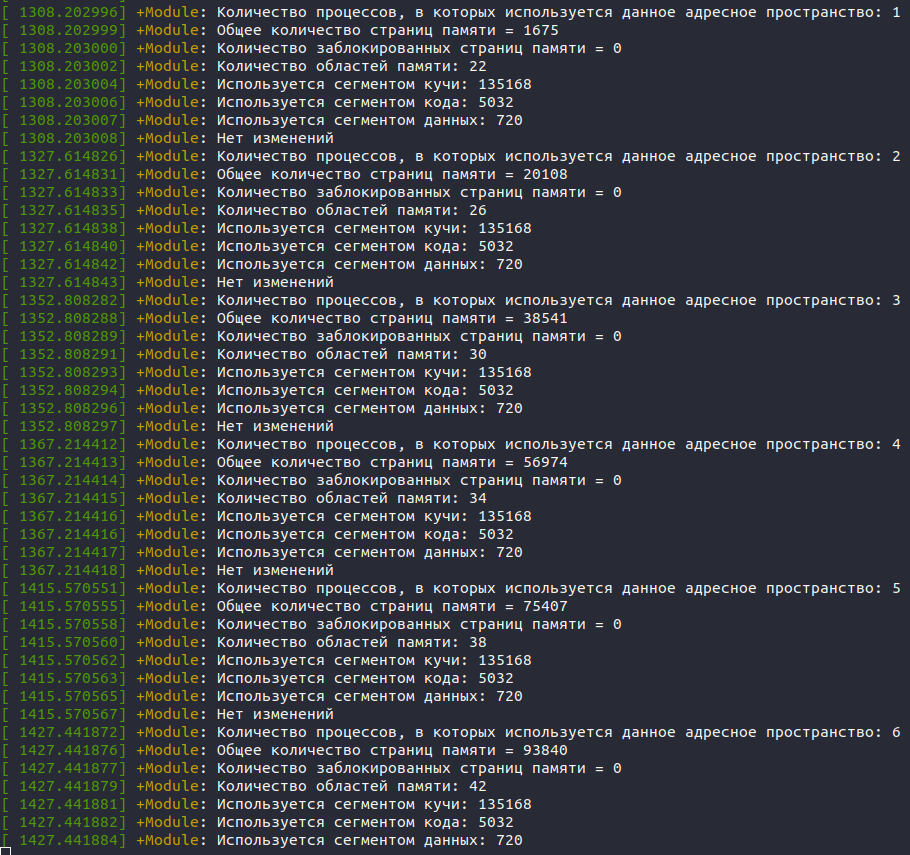
\includegraphics[width=0.95\textwidth]{img/analysis_pthread_count.png}
		\caption{Демонстрация увелечения количества страниц от количества потоков}
		\label{fig:analysis_pthread_count}}
\end{figure}

\newpage

// TODO: Указать размер  выделяемой памяти

\section{Анализ увелечения количества страниц программы, описанной выше}

На рис. \ref{fig:analysis_program} демонстрируется увеличение количества страниц 
при анализе описанной выше программы (при одном потоке).

Видно, что программе выделяется 33 страницы. 
Так же видно, что увеличивается размер кучи. 
Он увеличивается на 135168, что равно 33 * 4 * 1024, т.е. все 33 страницы выделяются под кучу.

\begin{figure}[ht!]
	\centering{
		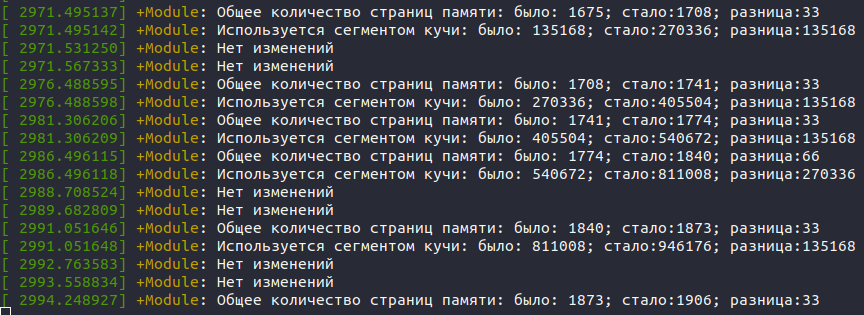
\includegraphics[width=1\textwidth]{img/analysis_program.png}
		\caption{Демонстрация увеличение количества страниц при анализе описанной выше программы}
		\label{fig:analysis_program}}
\end{figure}

\newpage

\section{Анализ увелечения количества страниц программы, описанной выше при увеличении количества потоков}

На рис. \ref{fig:analysis_program2} демонстрируется увеличение количества страниц 
при анализе описанной выше программы при увеличении количества потоков от 1 до 4.

Видно, что независимо, от изначального количества потоков программе выделяется 33 страницы. 

\begin{figure}[ht!]
	\centering{
		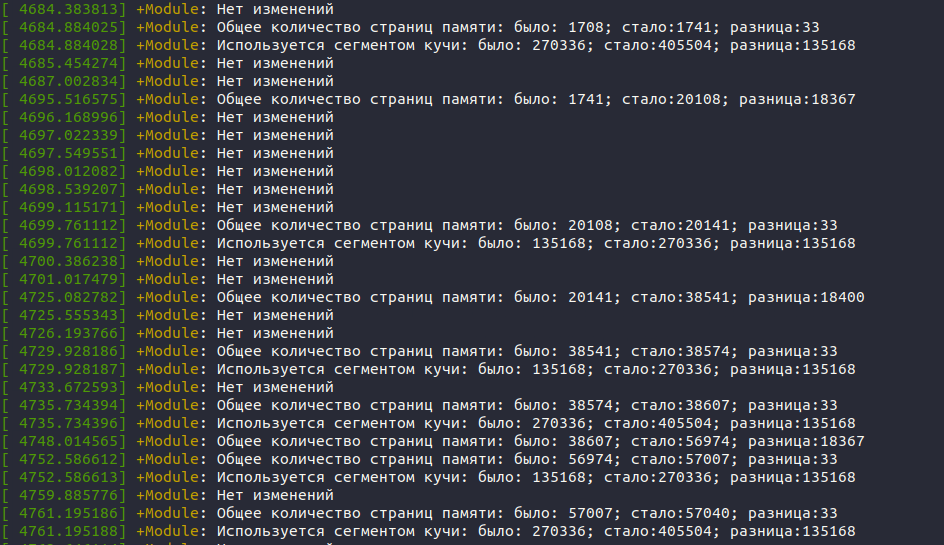
\includegraphics[width=1\textwidth]{img/analysis_program2.png}
		\caption{Демонстрация увеличение количества страниц при анализе описанной выше программы при увеличение кол-ва потоков}
		\label{fig:analysis_program2}}
\end{figure}

\section{Вывод}

В данном разделе был приведен анализ описанной выше программы.